\chapter{Estado de la cuestión}

Hoy en día contamos con microcontroladores y  ordenadores embebidos de muy bajo coste. Soluciones como Raspberry PI \cite{raspberrypi}, Beaglebone \cite{beaglebone}, o Arduino \cite{arduino} son claros ejemplos de hardware de bajo precio y alta calidad, la cual nos permite realizar proyectos de integración hardware entre dispositivos de una forma sencilla.

Uno de los problemas que nos podemos encontrar con el desarrollo de cualquier solución tecnológica son los problemas derivados de trasladar una idea de negocio o proyecto a un producto finalizado, que funcione de forma adecuada, sea estable y que realice exactamente lo definido.

Un problema común en la mayoría de desarrollo software, debido a que no existe una comunicación entre el diseño de la aplicación y su implementación, desarrollándola utilizando diseños estáticos, donde una modificación no pasa a las siguientes fases de desarrollo.

Esto es debido a que el desarrollo de software no se realiza de la misma forma que se realiza otro producto, donde existe una fase de diseño y otra de desarrollo totalmente diferenciadas. 
El software es completamente manipulable, por lo que el propio desarrollo del software es en si mismo el diseño de este, pudiendo separar estos conceptos, más a bajo nivel, y definir una separación entre interfaces e implementaciones.

Como solución a todos estos problemas, surgen varias metodologías, entre ellas \gls{mde}, y dentro de esta la metodología \gls{mdsd}.

Mediante esta metodología, podemos definir unos modelos que especifiquen de forma abstracta cual va a ser la funcionalidad a cubrir, y mediante transformaciones de ellos, podremos especificar detalles cada vez de más bajo nivel o niveles de implementación como por ejemplo, el lenguaje a utilizar, el \gls{framework} de este lenguaje, la plataforma de despliegue, o incluso los \glspl{script} de despliegue.

Una ventaja respecto a otros sistemas, es que no es un proceso en el que desarrollamos un único modelo y a partir de el realizamos una implementación, sino que la propia implementación la realizamos nosotros mismos en base a transformaciones, con lo que siempre vamos a tener concordancia con el modelo y la transformación, contando así con ventajas como:

\begin{itemize}

    \item Una documentación fiable, exacta al modelo.
    \item Separación del dominio e implementación.
    \item Test unitarios y de integración derivados del modelo.
\end{itemize}



%https://link.springer.com/chapter/10.1007/978-3-319-39110-6_6

%https://www.zephyrproject.org/


\section{MDA - Arquitectura dirigida por modelos}

La arquitectura dirigida por modelos \gls{mda}, es una iniciativa originariamente propuesta por el \gls{omg}.

\gls{mda}  \cite{mda_distilled} define un sistema de arquitectura software basado en cuatro capas (detalle en tabla \ref{tab:capas_mda})  cada una de ellas en un nivel de abstracción diferente.

\begin{table}[]
\centering
\begin{tabular}{@{}lll@{}}
\toprule
Capa & Nombre            & Ejemplo                                 \\ \midrule
M3   & Meta metamodelado & MOF                                     \\
M2   & Metamodelo        & UML / Ecore                             \\
M1   & Modelo            & Clases, estructuras de datos, funciones \\
M0   & Instancia         & Datos instanciados                      \\ \bottomrule
\end{tabular}
\sourcepropia{}
\caption{Diferentes capas de la arquitectura MDA}
\label{tab:capas_mda}

\end{table}




MDA utiliza en parte los siguientes estándares: 
\begin{itemize}
    \item \gls{uml} \cite{uml}
    \item \gls{mof} \cite{mof}
    \item \gls{xmi} \cite{xmi}
    \item \gls{edoc} \cite{edoc}
    \item \gls{spem} \cite{spem}
    \item \gls{cwm} \cite{cwm}
\end{itemize}


\subsection{Modelos}

Dentro de \gls{mda}, un modelo es un conjunto de elementos utilizados para representar una entidad en un nivel de abstracción determinado.

Un modelo puede estar representado de forma textual o de forma gráfica mediante una serie de diagramas interrelacionados.

\subsection{Meta-Modelos}
Un meta modelo \cite{mda_distilled_intro}, es un modelo del lenguaje, el cual define las relaciones, semántica, usos, restricciones de una serie de modelos.

\subsection{Plataformas}

\gls{mda} utiliza los conceptos \gls{cim}, \gls{pim} y \gls{psm}. \cite{mda_wirtschaftsinformatik}

\gls{cim} es una representación del sistema sin especificar como estará implementada en un sistema informático. Podríamos tomar como ejemplo de un \gls{cim}, el lenguaje de modelado \gls{bpmn}.

Mediante el \gls{pim}, normalmente definido en \gls{uml} con anotaciones, representamos un modelo el cual es independiente de la plataforma despliegue. La idea principal con este concepto es la transformación de esta representación a una o varias representaciones \gls{psm}, específicas para una plataforma determinada. 

Uno de los estándares que define \gls{mda} para realizar la transformación se denomina \gls{qvt}.

Por último contamos con \gls{psm}, el cual es un modelo ejecutable en una plataforma especifica. En el caso de \gls{mda}, puede estar definido por anotaciones específicas de \gls{uml}, tales como UML executable \cite{uml_executable}, o de otras plataformas de generación de código tales como \gls{ecore} / xtext.


\section{Lenguajes específicos de dominio}

Los lenguajes específicos de dominio \gls{dsl} nos permiten abstraernos de las peculiaridades con la implementación y centrarnos en definir nuestro producto en un lenguaje más cercano al dominio de negocio utilizado, por ejemplo los sistemas conectados a internet basados en arquitecturas Raspberry o Arduinio.

Para ello, nos es muy útil contar con un lenguaje de definición en el que podamos asignar eventos a actuaciones, ya sean locales o remotas, sin tener que entrar en como son capturados estos eventos, o como son realizadas dichas actuaciones.

\subsection{Eclipse EMF}

\gls{emf} \cite{EclipseEMF} es un \gls{framework} de modelado y meta-modelado que extiende de la funcionalidad proporcionada por el \gls{ide} Eclipse.
Este \gls{framework} introduce el concepto de modelos \gls{ecore}, modelos similares a clases de un lenguaje de programación común, con el añadido de la creación de editores y visualizadores de los datos generados a partir de dichos modelos.

Los modelos \gls{ecore}, proporcionan funcionalidad básica en la generación de clases para el lenguaje Java,  la  edición de modelos mediante el propio \gls{ide} Eclipse, la creación de test unitarios, así como la personalización en la generación de todo este código.

Mediante la utilización del propio editor integrado, aseguramos la correcta generación y construcción de los modelos. En la figura \ref{fig:estado_ecore_ejemplo1} podemos observar la definición de modelo y en la siguiente figura \ref{fig:estado_ecore_ejemplo2} mostramos la edición de una instancia de datos generados a partir de un modelo \gls{ecore}.





\begin{figure}
	\centering
    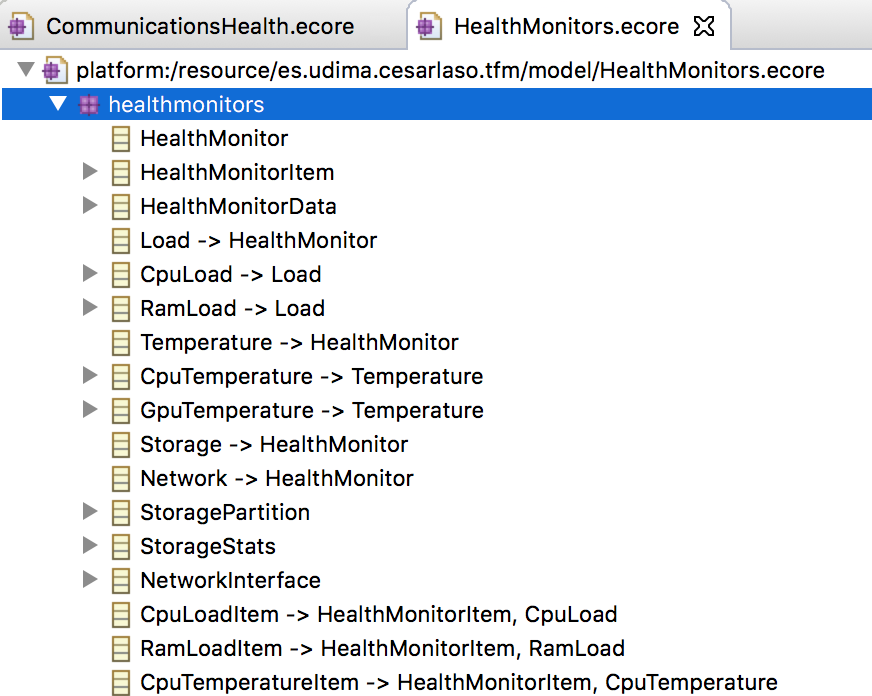
\includegraphics[scale=0.4]{images/estado_cuestion/ecore_ejemplo1.png}
    \sourcepropia{}
    \caption[Definición de un modelo \gls{ecore} en formato tree]{Definición de un modelo \gls{ecore} en formato tree. En este tipo de visualización podemos ver la herencia de los modelos, los interfaces que implementa, y en caso de desplegar los elementos del árbol, sus atributos.}
    \label{fig:estado_ecore_ejemplo1}
\end{figure}

\begin{figure}
	\centering
    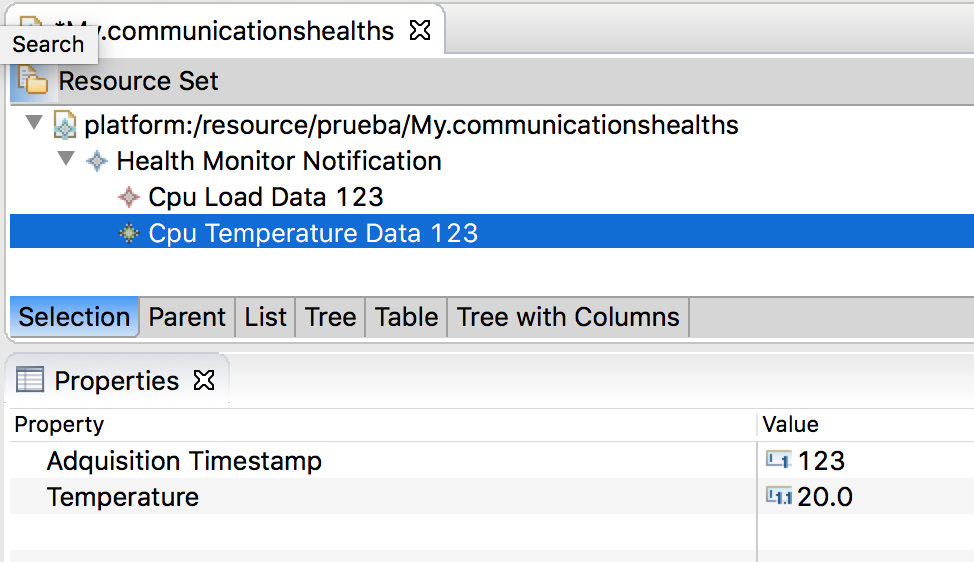
\includegraphics[scale=0.4]{images/estado_cuestion/ecore_ejemplo2.png}
    \sourcepropia{}
    \caption[Edición de una instancia generada a partir de un modelo \gls{ecore} en su formato de visualización tree]{Edición de una instancia generada a partir de un modelo \gls{ecore} en su formato de visualización tree. Esta visualización es personalizable en textos e iconos, permitiendo desarrollar editores muy alineados con la temática del negocio. El editor ejecuta las reglas de validación de los atributos, mostrando los tipos de datos permitidos para cada uno de ellos y mostrando error en caso de valores no permitidos tanto por el tipo de dato, como por la validación adicional que indiquemos.}
    \label{fig:estado_ecore_ejemplo2}
\end{figure}


\gls{ecore} gestiona la persistencia de sus datos mediante archivos \gls{xml}, con lo que podemos editarlos de forma textual si fuera necesario sin necesidad de contar con el propio \gls{ide}. La figura \ref{fig:estado_ecore_xml} muestra uno de los modelos en su formato \gls{xml}, el cual posteriormente comentaremos en el desarrollo del proyecto.


\begin{figure}
	\centering
	
	\lstinputlisting[language=xml,caption={}]{ejemplos/estado_cuestion_events.ecore}
	
    \sourcepropia{}
    \caption{Representación \gls{xml} del modelo \gls{ecore} Events}
    \label{fig:estado_ecore_xml}
\end{figure}






\subsection{Xtext}

Para este trabajo, utilizaremos el kit de desarrollo \gls{xtext} \cite{xtext}.

Este producto, cuenta con una infraestructura completa de desarrollo de lenguajes tipados,  incluyendo parser, linker, checkeador de tipos de datos, compilador y editor tanto de escritorio (basado en eclipse EMF), como online a través de un navegador web online. Ver figura \ref{fig:xtext_editor_eclipse_dsl}.

\begin{figure}
	\centering
    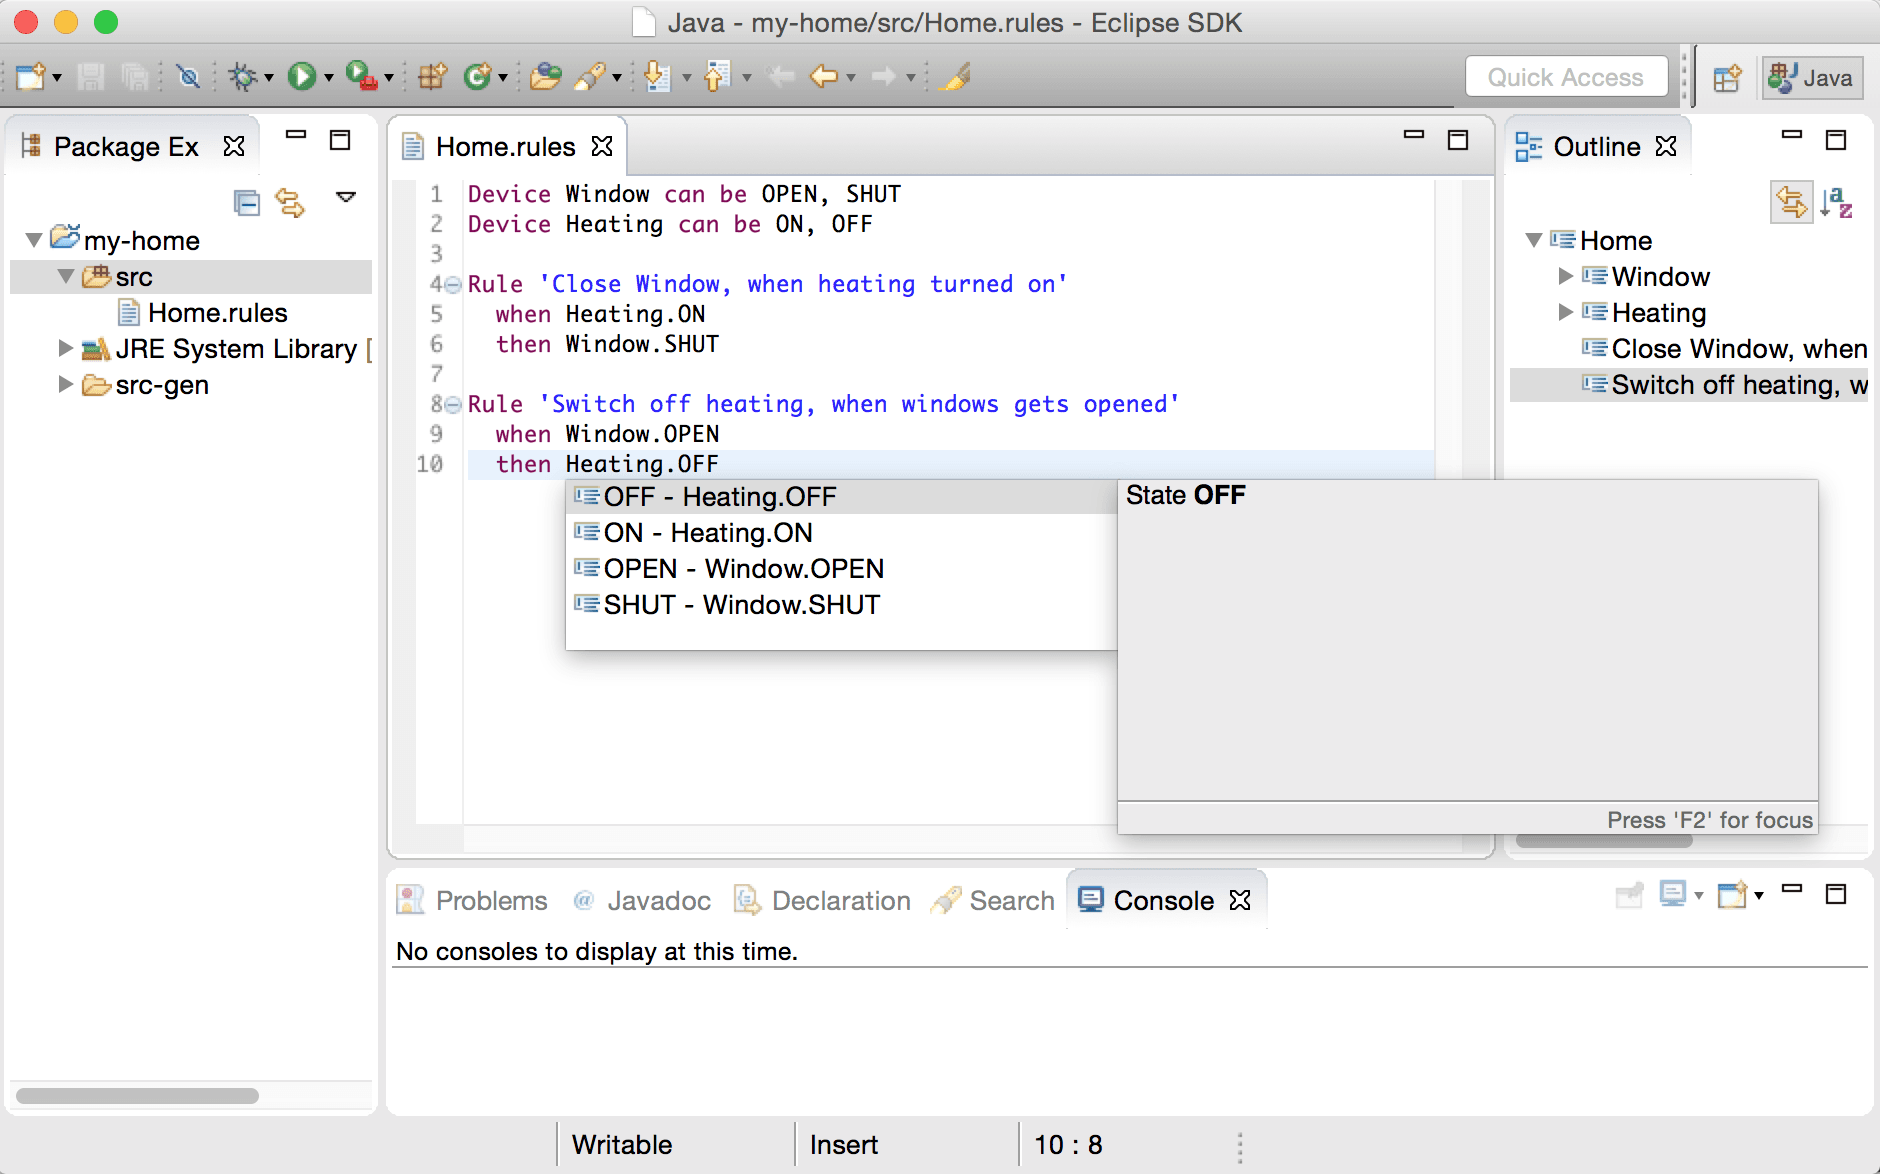
\includegraphics[height=0.3\textheight]{images/estado_cuestion/xtext_screenshot.png}
    \source{Web Xtext \cite{xtext}}
    \caption[IDE Eclipse con Xtext editando DSL]{IDE Eclipse con Xtext editando DSL con soporte de tipado y autocompletado. El editor muestra el programa como si de un lenguaje de programación general se tratara, con todas las ventajas que aporta.}
    \label{fig:xtext_editor_eclipse_dsl}
\end{figure}

El posterior desarrollo del \gls{dsl}, lo realizaremos utilizando esta herramienta, ya que nos proporciona todo lo que vamos a necesitar para realizar un \gls{dsl} que cumpla con nuestras necesidades.

Esta herramienta es de gran calidad y es utilizada tanto en investigación como en desarrollo de proyectos industriales por empresas como la \gls{esa}, BOSCH, Siemens o SAP \cite{xtext}


\subsection{MPS}

Otra herramienta de especial mención es MPS \cite{mps}, de Jetbrains \cite{jetbrains}.

Esta herramienta, basada en el \gls{ide} IntelliJ \cite{intellijidea}, cuenta al igual que Xtext, con todas las herramientas necesarias (ver figura \ref{fig:mps_editor_dsl}) para el desarrollo de lenguajes específicos de dominio, tales como compilador, parseador, linker, editor.

\begin{figure}
	\centering
    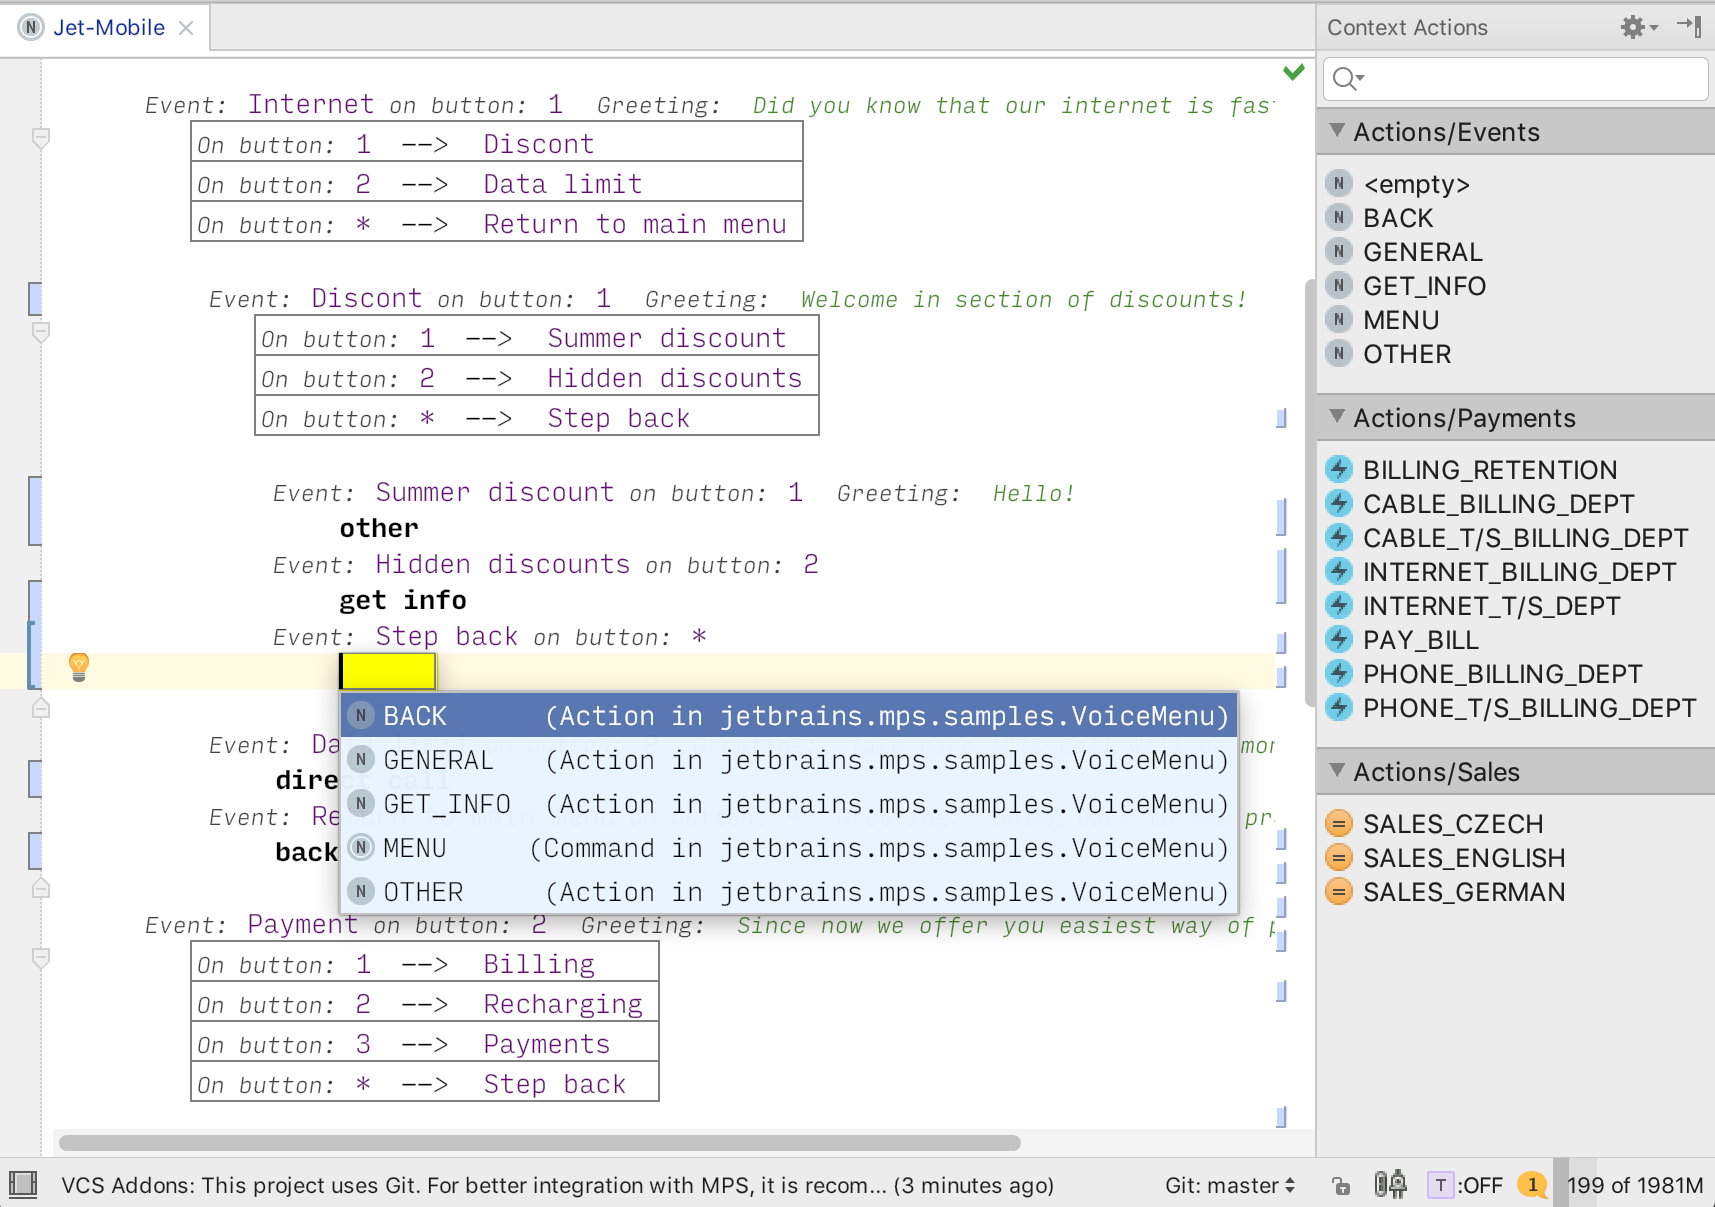
\includegraphics[height=0.3\textheight]{images/estado_cuestion/mps-language-support.png}
    \source{Web MPS \cite{mps}}
    \caption[IDE MPS editando un DSL]{IDE MPS editando en un DSL con soporte de autocompletado. Soporta todas las opciones de refactorización que incluye el IDE en el que esta basado IntelliJ}
    \label{fig:mps_editor_dsl}
\end{figure}

Los aspectos destacables de esta herramienta son una integración completa con el editor IntelliJ, soporte profesional por parte de la empresa Jetbrains e incluso formación en la herramienta y desarrollo del lenguaje.

El software cuenta con la licencia OpenSource Apache 2.0. \cite{mps_licencia}.


Cuenta con soporte de generación de código basado en la \gls{jvm} y cuenta con soporte de terceros para C, .NET y javascript.

Mención especial merece la aplicación mbeddr \cite{mbeddr} basada en MPS,  la cual incluye incluso herramientas de  verificación y validación de software tal como podemos observar en la figura  \ref{fig:mbeddr_editor_dsl}.

\begin{figure}
	\centering
    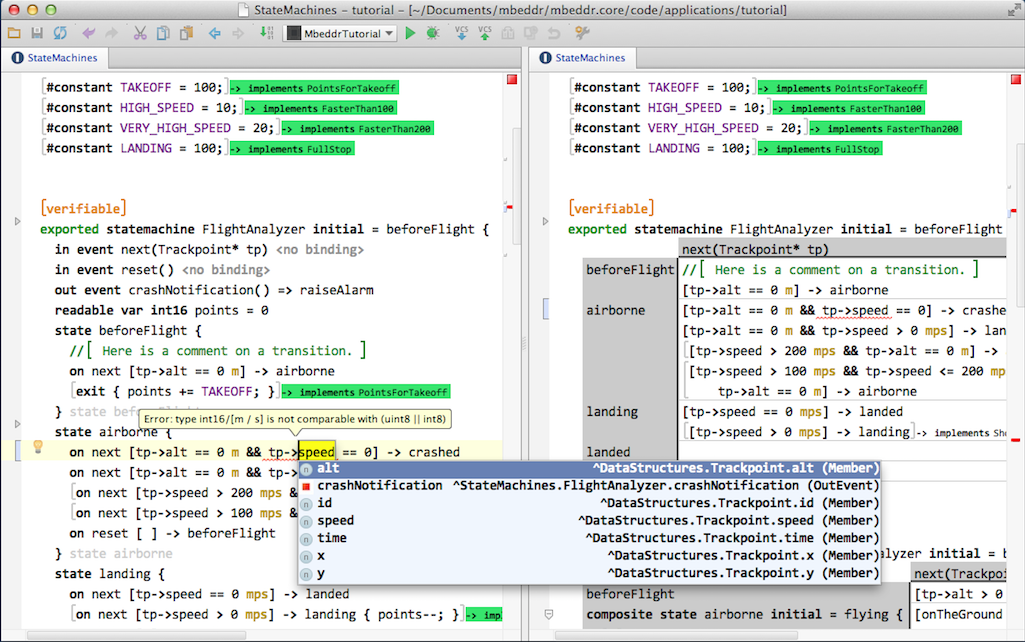
\includegraphics[height=0.3\textheight]{images/estado_cuestion/mbeddr_editor.png}
    \source{Web mbeddr \cite{mbeddr}}
    \caption[IDE MBEDDR]{IDE MBEDDR editando en un DSL con soporte de verificación y validación.}
    \label{fig:mbeddr_editor_dsl}
\end{figure}




\section{Trabajos relacionados}

\subsection{DSL for arduino}

%Koopman y Plasmeijer 
\textcite{shallow_embedded_dsl_arduino} crearon una plataforma similar a la de este trabajo, la cual define un \gls{dsl}, el cual nombran como ARDSL que compila a código C++ para la plataforma Arduino UNO.

En este caso, el \gls{dsl} está creado a partir del lenguaje de programación funcional Clean \cite{clean_lang}.

A continuación podemos ver en la figura \ref{fig:dsl_for_arduino} un ejemplo de código implementado en el \gls{dsl} .

\begin{figure}
	\centering
	
	\lstinputlisting[caption={}]{ejemplos/estado_cuestion_shallow_dsl_arduino_ejemplo.txt}
	
    \sourcepropia{}
    \caption[DSL for Arduino ejemplo fragmento código]{DSL for Arduino, ejemplo de código donde cada 500 ms se alterna el estado de un led. El lenguaje creado es muy cercano tanto al modelo de negocio como a un lenguaje de proposito general.}
    \label{fig:dsl_for_arduino}
\end{figure}


\subsection{OpenHab}

OpenHab \cite{openhab} es un programa completo para el control de elementos conectados a internet, con soporte para múltiples plataformas y dispositivos \gls{iot}.

Este producto utiliza el mismo lenguaje de creación de \gls{dsl} que este trabajo, el lenguaje Xtext para definir un \gls{dsl} propio, en este caso utilizado para la gestión de máquinas de estado y reglas lógicas entre dispositivos.

Este producto, al ser un producto de consumidor final, tal como definen desde su propia web, cuenta con las siguientes ventajas:


\begin{itemize}
    \item Diseñado para ser neutral respecto al fabricante, y frente al protocolo.
    \item Corre en cualquier dispositivo que sea capaz de ejecutar la \gls{jvm}.
    \item Cuenta con un motor de reglas adaptado a la automatización.
    \item Cuenta con interfaces web y nativo iOS / Android.
    \item Código abierto, comunidad abierta.
    \item Proporciona APIs de integración.
\end{itemize}


Se muestra un ejemplo de configuración de este entorno en la figura \ref{fig:openhab_ejemplo}.

\begin{figure}
	\centering

    \lstinputlisting[caption={}]{ejemplos/estado_cuestion_openhab_ejemplo.txt}

    \source{Openhab \cite{openhab}}
    \caption[Openhab reglas ejemplo]{Fragmento de código en la definición de reglas Openhab. En el ejemplo se modifica un actuador, luces del salón, en función de un evento, estado de la reproducción del televisor}
    \label{fig:openhab_ejemplo}
\end{figure}
